\section{Numerical Results}

We validate our  algorithmic insights and then our theory.
In Section \ref{sec_exp_res}, we first show that single-task learning results can help predict positive or negative transfer.
%the single-task based metric on sentiment analysis and ChestX-ray14 datasets.
Second, our proposed incremental training schedule improves the training efficiency of standard multi-task training on sentiment analysis tasks.
%Third, we measure the data efficiency ratio of multi-task learning on six sentiment analysis tasks.
In Section \ref{sec_exp_ab}, we validate our theoretical results.
We further show that when the sample ratio is large, performing the alignment procedure of \cite{WZR20} provides more improvement for MTL.

\begin{table}[!b]
%\begin{minipage}[t]{.58\textwidth}
%	\vspace{-0.1in}
%	\centering
%  \begin{tabular}{c c c c c}
%	\toprule
%		\multirow{2}{*}{{\bf Threshold}}  & \multicolumn{2}{c}{{\bf Sentiment
%		analysis}} & \multicolumn{2}{c}{{\bf ChestX-ray14}} \\
%		& Precision &  Recall & Precision &  Recall \\
%		\cmidrule(lr){1-1} \cmidrule(lr){2-3} \cmidrule(lr){4-5}
%		0.0 & 0.596 & 1.000 & 0.593 & 1.000 \\
%		0.1 & \textbf{0.756} & \textbf{0.388} & \textbf{0.738} & \textbf{0.462} \\
%		0.2 & 0.919 & 0.065 & 0.875 & 0.044 \\
		% 0.3 & 1.000 & 0.004 &     - &     - \\
%	\bottomrule
%	\end{tabular}
%	\vspace{0.1in}
%	\captionof{table}{Single-task learning results can help predict postive or negative transfer in multi-task learning.}
%	\label{tab:mtl_better_than_stl}
%\end{minipage}%
%\quad
	\begin{minipage}[t]{.40\textwidth}
	\vspace{-0.1in}
	\centering
	\begin{tabular}{c c c}
		\toprule
		% \multirow{2}{*}{{\bf Models}} & \multicolumn{2}{c}{\begin{minipage}{1.2in}\begin{center}
		% Sentiment\\ analysis\end{center}\end{minipage}} \\
		\multirow{2}{*}{{\bf Models}} & \multicolumn{2}{c}{\bf Sentiment analysis} \\
		% \cmidrule(lr){2-3}
		& all tasks & w/o TREC \\
		\midrule
		{\bf MLP}  & 31\% & 29\% \\
		{\bf LSTM} & 35\% & 34\% \\
		{\bf CNN}  & 30\% & 28\% \\
		\bottomrule
		\end{tabular}
	\vspace{0.1in}
	\captionof{table}{Efficiency of incremental training compared to baseline MTL.}
	\label{tab:taskonomy}
\end{minipage}
\end{table}

\subsection{Experimental Setup}

We consider a text classification task and an image classification task as follows.

{\it Sentiment Analysis.} We consider six tasks: movie review sentiment (MR) \cite{pang2005seeing}, sentence subjectivity (SUBJ) \cite{pang2004sentimental}, customer reviews (CR) \cite{hu2004mining}, question type (TREC) \cite{li2002learning}, opinion polarity (MPQA) \cite{wiebe2005annotating}, and the Stanford sentiment treebank (SST) tasks \cite{socher2013recursive}.
%The question is to predict positive or negative sentiment expressed in the text.
We use an embedding layer with GloVe embeddings \cite{pennington2014glove}
followed by an LSTM, MLP or CNN layer proposed by~\cite{lei2018simple}.

%multi-layer perceptron (MLP), LSTM, CNN on all tasks
%We use this task to verify our theoretical results on model capacity and task covariance in real world.

{\it ChestX-ray14.} This dataset contains 112,120 frontal-view X-ray images \cite{chexnet17}.
There are 14 diseases (tasks) for every image that we would like to predict.
We use densenet121 as the shared module \cite{huang2017densely}.
%We treat each label as one task a binary classification problem and formulate it as a 14-task multi-task learning problem.
%This dataset is curated where the labels
%We use the CheXNet model from~\cite{chexnet}, which is a 121-layer convolutional neural network on all tasks.

\paragraph{Synthetic Settings}\label{app_synthetic}
	We describe the parameter settings used in the synthetic experiments (Figure \ref{fig_model_shift_phasetrans}).
	For all three synthetic experiments, we set the input feature dimension as $p = 200$.
	\squishlist
		\item Task similarity: We use $\rho_1 = 90, \rho_2 = 30$ for sample sizes.
	The noise level is $\sigma = 5$.
	We set $\kappa = 1$ and vary model distance $d$ from $0.01$ to $0.2$.
	The $x$-axis measures the function $\Phi(\beta_1, \beta_2)$ described in Section \ref{sec_similarity}.
	The $y$-axis measures the improvement of prediction loss using MTL compared to STL.
		\item Sample size: We set $\kappa = 1$ and $d = 0.02$ for model distance.
	We use $\rho_2 = 500$ and vary $\rho_1$ from $50$ to $800$ for sample sizes.
		\item Covariate shift: We set $\kappa = 1$ and $d = 0$.
	We set $\rho_2 = 4$ and vary $\rho_1$ from $5$ to $25$ for sample sizes.
	We use the scale parameter $\lambda = 1$ for the curve without covariate shift and $\lambda = 2$ for the curve with covariate shift (cf. Section \ref{sec_covshift}).
	Without loss of generality, we have rescaled the $x$ and $y$ axis for the ease of presentation.
	This can be achieved similarly by rescaling the task data.
	\squishend

\paragraph{Image and Text Classification Settings}\label{app_it}

For the text classification experiment, we encode each word using the GLoVe word embeddings.%
\footnote{http://nlp.stanford.edu/data/wordvecs/glove.6B.zip}
We evaluate three model choices.
For multi-layer perception (MLP), we apply an average pooling layer over the word embeddings.
For LSTM and CNN, we add a shared feature representation layer on top of the word embeddings \cite{lei2018simple}.

\textit{Predicting transfer effect via STL results.}
We simplify the setup of this experiment by fixing the sample sizes of every task pair.
For sentiment analysis tasks, the sample size of the source task ranges in $500, 1000, 1500$.
We randomly sample these many data points from the task.
The sample size of the target task is $1000$.
For image classification tasks, the training sample size is $10,000$ for every task.

\textit{Mitigating negative transfer via incremental training.}
For the case of two tasks, we compare the incremental training scheduled described in Algorithm \ref{alg_inc_train}  to a round-robin training schedule baseline.
We add $20\%$ of source task samples for every $T = 2$ epochs.
The total number of epochs is $20$.
We set the threshold $\tau$ as the validation accuracy of the target task using the baseline training schedule.

For the case of six tasks, we extend Algorithm \ref{alg_inc_train} accordingly.
Initially, we use $5\%$ of samples from SST and $50\%$ of samples from the other tasks.
We add $19\%$ of samples from SST and $5\%$ of samples from the other tasks for every $2$ epochs.
We run $20$ epochs in total.
%\textbf{The training procedure and baseline.}
For all models, we use a shared module for all tasks and assign a separate output layer on top of the shared module for each task.
The baseline training schedule for MTL is the round-robin training schedule.
%We compare our incremental training schedule of Algorithm \ref{alg_inc_train} to the round-robin training schedule.
We measure the test accuracy of predicting a target task.
We measure computational cost by summing over all epochs the number of samples used in every epoch.

\textit{Validating the Theoretical Results.}
We fill in the details of the experimental procedure used for the results in Figure \ref{fig_ablation}.
\squishlist
	\item Task similarity: We select a similar and a dissimilar source task compared to the target task using domain knowledge.
First pair: the customer review dataset (CR) , which predicts whether a review is positive or negative, is more similar to SST (sentiment treebank) than MPQA (question type).
Second pair: SST is more similar to MR since they both concern about positive or negative opinions expressed the text.
TREC is less similar to MR because the task is about question types.
Third pair: MPQA (opinion polarity) is more similar to TREC (question type)
	\item Sample size: We vary the sample size of the source task from $100$ to $3000$.
	\item Covariate shift: We implement the covariance alignment procedure following \cite{WZR20}.
	We fix the sample size of the target task as $1000$.
\squishend

%\subsection{Validating the Theoretical Results}\label{sec_exp_ab}
%We first validate our theoretical results in Section \ref{sec_similarity} and \ref{sec_data_size}.
%In Figure \ref{fig_ab_sim}, we compare the performance training with a semantically similar task versus a dissimilar task with a target task.
%We select each task pair based on our domain knowledge.
%We observe that adding a similar task helps the target task whereas adding a dissimilar task hurts.
%The rest of experimental procedures are left to Appendix \ref{app_it}.

\subsection{The Same Covariates Setting: Sample Efficiency}

%We validate that MTL performs better when the source task is more similar to the target task.
%We show the result on the sentiment analysis tasks.
%For a target task, we manually select a similar task and a dissimilar task based on prior knowledge.
%Figure \ref{fig_ab_sim} confirms the result.
%Recall that Section \ref{sec_data_size} shows that increasing the data size of the source task does not always improve the performance of MTL for the target task.
%In Figure \ref{fig_ab_data}, we show that for source task MR and target task SST, there is a transition from positive to negative transfer as we increase the data size of the source task.
%Our result provides a fine-grained insight on the covariance alignment algorithm proposed in \cite{WZR20}.
%Recall that the covariance alignment procedure in \cite{WZR20} adds an additional module between the word embedding representation and the shared module.
%When the source task data size is particularly large compared to the target task, we show that applying the covariance alignment algorithm results in more significant gains.
%In Figure \ref{fig_ab_cov}, we observe that the benefit from aligning task covariances becomes more significant for LSTM and MLP as we increase the number of datapoints of the source task.

\begin{table}
	\begin{center}
		\begin{tabular}{c c c c c}
			\toprule
			\multirow{2}{*}{{\bf Models}} & \multicolumn{2}{c}{\begin{minipage}{1.1in}\begin{center}
				                                                                          MR, SST, SUBJ, CR, MPQA, TREC\end{center}\end{minipage}} & \multicolumn{2}{c}{\begin{minipage}{1.1in}\begin{center}MR, SST, SUBJ, CR, MPQA\end{center}\end{minipage}} \\
			\cmidrule(lr){2-3} \cmidrule(lr){4-5}
			& {\bf Stanford} & {\bf Alignment} & {\bf Stanford} & {\bf Alignment} \\
			\midrule
			{\bf MLP}  & > 100\% & 39\% & 25\% & 25\% \\
			{\bf LSTM} & 36\% & 36\% & 28\% & 25\% \\
			% {\bf CNN}  & 76\% & - & 32\% & -\\
			\bottomrule
		\end{tabular}
	\end{center}
	\caption{Taskonomy experiment.}
	\label{tab:taskonomy}
\end{table}


\begin{figure}[!t]
	\begin{subfigure}[b]{0.32\textwidth}
		\centering
		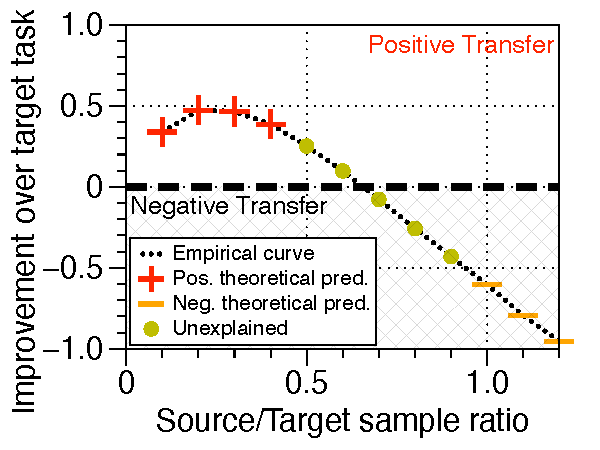
\includegraphics[width=0.98\textwidth]{figures/datapoints_phase_transition.pdf}
		\caption{Sample imbalance}
		\label{fig_size}
	\end{subfigure}\hfill
	\begin{subfigure}[b]{0.32\textwidth}
		\centering
		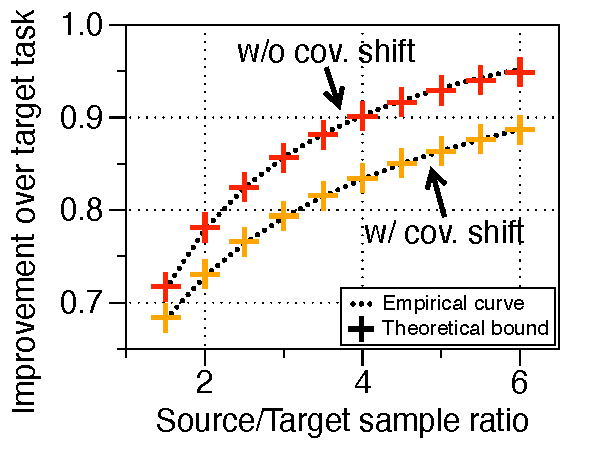
\includegraphics[width=0.98\textwidth]{figures/complementary.pdf}
		\caption{Covariate shift}
		\label{fig_covariate}
	\end{subfigure}\hfill
	\begin{subfigure}[b]{0.32\textwidth}
		\centering
		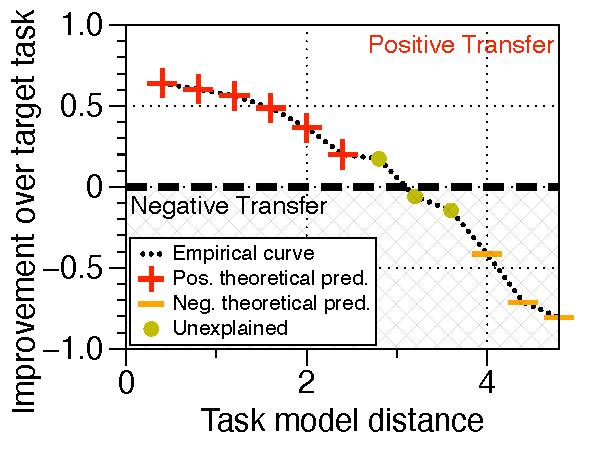
\includegraphics[width=0.98\textwidth]{figures/model_shift_phase_transition.pdf}
		\caption{Sample efficiency}
		\label{fig_model_shift}
	\end{subfigure}
	\caption{%Three takeaways of our theory in Section \ref{sec_insight}.
	We observe a transition from positive to negative transfer as (a) \textit{task model distance} increases and (b) source/target \textit{sample ratio} increases.
	For the special case of having the same task model, we observe in (c) that as source/target \textit{sample ratio} increases, having \textit{covariate shift} worsens the performance of MTL.
	The $y$-axis measures the loss of STL minus MTL.}
	\label{fig_model_shift_phasetrans}
\end{figure}


\subsection{The Different Covariates Setting: Sample Imbalance and Covariate Shift}\label{sec_exp_sample}

%\textit{Predicting transfer effect via STL results.}
%We show that the single-task based metric proposed in Section \ref{sec_similarity} can predict positive or negative transfer in MTL.
%A common challenge in the study of MTL is that the results can be hard to understand.
%It is difficult to predict when MTL performs well without running extensive trials.
%Our insight is that we can use STL results to help understand MTL results.
%Table \ref{tab:mtl_better_than_stl} shows the result on both the sentiment analysis and the ChestX-ray14 tasks.
%We find that using a threshold of $\tau = 0.1$, the STL results correctly predict positive or negative transfer with $75.6\%$ precision and $38.8\%$ recall among $30$ times $5$ (random seeds) task pairs!
%We observe similar results for $91$ task pairs from the ChestX-ray14 dataset.
%The results show that STL results are indicative of MTL results.

In Figure \ref{fig_ab_data}, we validate that adding more source samples does not always improve performance on the target task.
Finally, we validate the algorithmic consequence of Section \ref{sec_covshift}.

\textit{Mitigating negative transfer via incremental training.}
\noindent\textit{Mitigating negative transfer.}
An interesting consequence of Proposition \ref{prop_data_size} is that $L(\hat{\beta}_t^{\MTL})$ is not monotone in $\rho_1$.
In particular, Figure \ref{fig_size} (and our analysis) shows that $L(\hat{\beta}_t^{\MTL})$ behaves as a quadratic function over $\rho_1$.
More generally, depending on how large $\Psi(\beta_1, \beta_2)$ is, $L(\hat{\beta}_t^{\MTL})$ may also be monotonically increasing or decreasing.
Based on this insight, we propose an incremental optimization schedule to improve MTL training efficiency.
\squishlist
	\item We divide the source task data into $S$ batches.
	For $S$ rounds, we incrementally add the source task data by adding one batch at a time.
	\item After training $T$ epochs, if the validation accuracy becomes worse than the previous round's result, we terminate.
	Algorithm \ref{alg_inc_train} in Appendix \ref{app_experiments} describes the procedure in detail.
\squishend

\begin{algorithm}[!t]
	\caption{An incremental training schedule for efficient multi-task learning with two tasks}
	\label{alg_inc_train}
	\begin{algorithmic}[1]
		\Input Two tasks $(X_1, Y_1)$ and $(X_2, Y_2)$.
		\Param A shared module $B$, output layers $W_1, W_2$ as in the hard parameter sharing architecture.
		\Req \# batches $S$, epochs $T$, task $2$'s validation accuracy $\hat{g}(B; W_2)$, a threshold $\tau\in(0,1)$.
		\Output The trained modules $B, W_2$ optimized for task $2$.
		\State Divide $(X_1, Y_1)$ randomly into $S$ batches: $(x^{(1)}, y^{(1)}), \dots, (x^{(S)}, y^{(S)})$.
		\For{$i = 1,\dots, S$}
			\For{$j = 1,\dots, T$}
				\State Update $B, W_1, W_2$ using the training data $\set{x^{(k)}, x^{(k)}}_{k=1}^i$ and  $(X_2, Y_2)$.
			\EndFor
			\State Let $a_i = \hat{g}(B; W_2)$ be the validation accuracy.
			\If{$a_i < a_{i-1}$ or $a_i > \tau$}
				\State \textbf{break}
			\EndIf
		\EndFor
	\end{algorithmic}
\end{algorithm}


First, we show that our proposed incremental training schedule (Algorithm \ref{alg_inc_train}) can help mitigate negative transfer for predicting a particular target task.
Over all $15$ pairs from the sentiment analysis tasks, we find that Algorithm \ref{alg_inc_train} requires only $45\%$ of the computational cost to achieve similar performance on the target task, compared to the MTL baseline.
Our insight is that since adding more samples from the source task does not always help, we can improve efficiency by adding source samples \textit{incrementally} during training.

%\textbf{Improving transfer learning training efficiency.}
%We show that Algorithm \ref{alg_inc_train} also applies to transfer learning settings.
%Compared to fine-tuning the source model on the target task, we show that our proposed method reduces the computional cost by \alert{$xx\%$}, without sacrificing accuracy.

Our next result shows the incremental training schedule applies to multiple tasks as well.
In Table \ref{tab:taskonomy}, we find that over all six sentiment analysis tasks, incremental training requires less than $35\%$ of the computational cost compared to baseline MTL training, while achieving the same accuracy averaged over all six tasks.
As a further validation, excluding TREC, we observe similar comparative results.
%The data efficiency ratio of using MLP is $100\%$ because the average performance of MTL is worse than the average of STL.
%We further show that applying incremental training helps reduce the data efficiency ratio to \alert{$xx\%$}.
%If TREC is not included, we see that only $25\%$ of the labeled data is needed.


\begin{figure}[!t]
	\centering
	\begin{subfigure}[b]{0.33\textwidth}
		\centering
		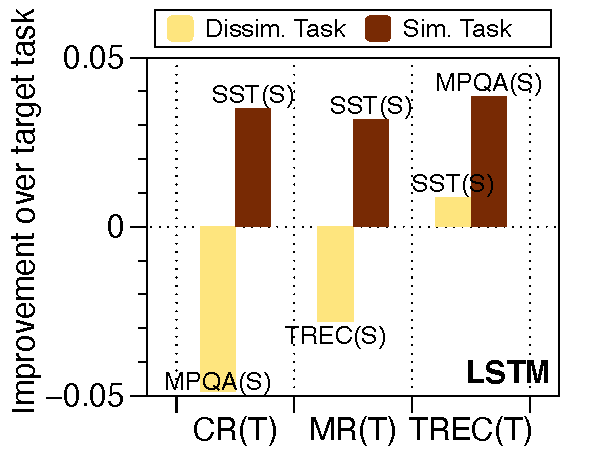
\includegraphics[width=0.975\textwidth]{figures/task_sim_norm_lstm.pdf}
		\caption{Task similarity}
		\label{fig_ab_sim}
	\end{subfigure}%
	\begin{subfigure}[b]{0.33\textwidth}
		\centering
		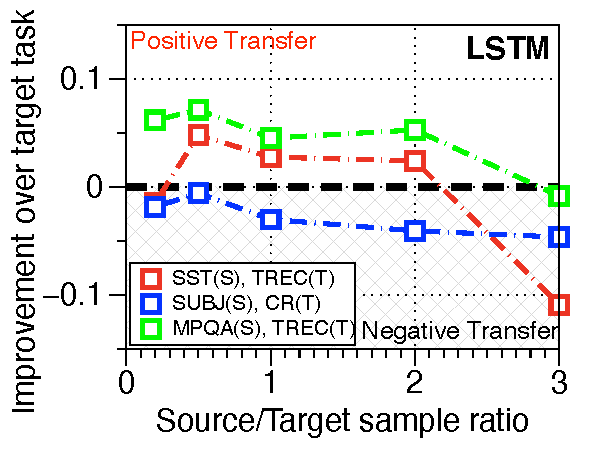
\includegraphics[width=0.975\textwidth]{figures/ratio_norm_3_pairs_lstm.pdf}
		\caption{Sample size}
		\label{fig_ab_data}
	\end{subfigure}
	\begin{subfigure}[b]{0.33\textwidth}
		\centering
		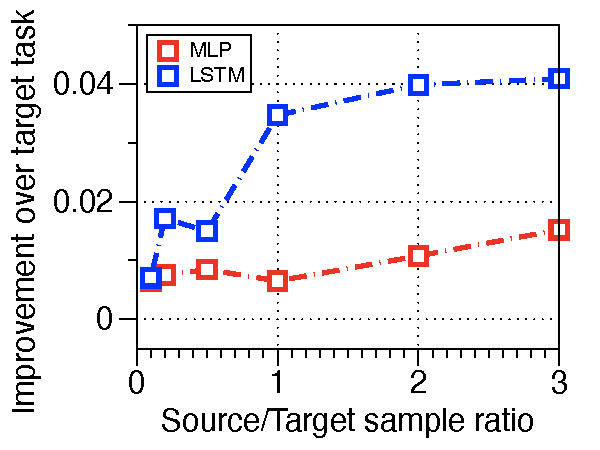
\includegraphics[width=0.975\textwidth]{figures/ratio_alignment_norm_diff_all.pdf}
		\caption{Covariate shift}
		\label{fig_ab_cov}
	\end{subfigure}
	\caption{Validating the three results of Section \ref{sec_insight} on sentiment analysis tasks. (a) Adding a semantically similar source task in MTL performs better than adding a dissimilar task.
	(b) As source/target sample ratio increases, we observe a transition from positive to negative transfer.
	(c) As source/target sample ratio increases, aligning task covariances \cite{WZR20} improves more over the baseline.
	Note: (S) denotes the source task and (T) denotes the target task.}
	\label{fig_ablation}
	\vspace{-0.15in}
\end{figure}





\noindent\textit{Covariance alignemnt.}
Our observation highlights the need to correct covariate shift when $n_1 / n_2$ is large.
Hence for such settings, we expect procedures that aim at correcting covariate shift to provide more significant gains.
We consider a covariance alignment procedure proposed in \cite{WZR20}, which is designed for the purpose of correcting covariate shift.
The idea is to add an alignment module between the input and the shared module $B$.
This new module is then trained together with $B$ and the output layers.
We validate our insight on this procedure in the experiments.


In Figure \ref{fig_ab_cov}, we measure the performance gains from performing the alignment procedure proposed in \cite{WZR20} minus baseline MTL.
We average the results over all 15 task pairs.
The result shows that as the source samples increases, the alignment procedure shows a bigger improvement over MTL.

\textbf{Further results of the covariance alignment procedure.}
Our results in Figure \ref{fig_ab_cov} are averaged over all the task pairs.
In Figure \ref{fig_covariate_app}, we show two task pairs as examples.
In Figure \ref{fig_cov_a}, we observe that for the particular task pair, covariance alignment provides more significant gains when the sample ratio is large.
In Figure \ref{fig_cov_b}, we observe that covariance alignment does not always improve over the baseline multi-task learning model.
One explanation is that MR and SST are similar tasks, hence adding the alignment module is unnecessary.
An interesting question is to understand when adding the alignment module benefits the multi-task learning model.
We leave this question for future work.
%Note: For text classification tasks, the source task training data size ranges from 500 to 1,500 and target task training data size is 1000; For ChestX-ray14,

\begin{figure}[!h]
	\centering
	\begin{subfigure}[b]{0.48\textwidth}
		\centering
		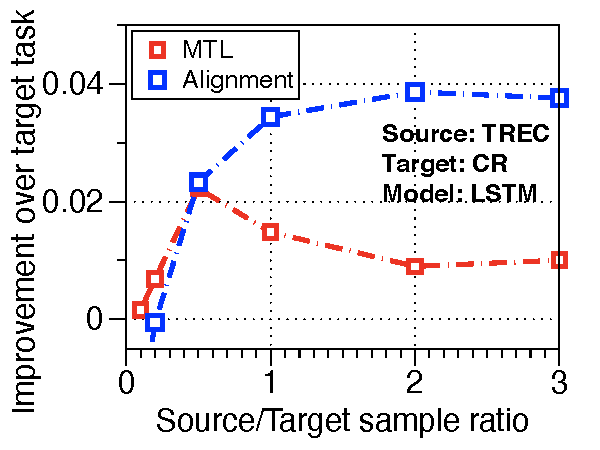
\includegraphics[width=0.7\textwidth]{figures/ratio_alignment_norm_trec_cr_lstm.pdf}
		\caption{Task pair TREC and CR}
		\label{fig_cov_a}
	\end{subfigure}\hfill
		\begin{subfigure}[b]{0.48\textwidth}
		\centering
		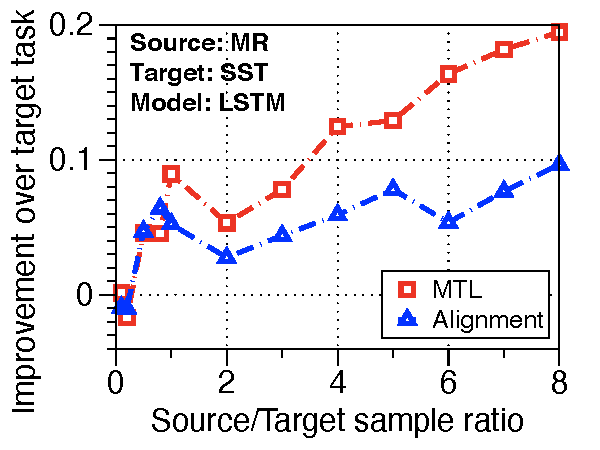
\includegraphics[width=0.7\textwidth]{figures/ratio_alignment_mr_sst_lstm.pdf}
		\caption{Task pair MR and SST}
			\label{fig_cov_b}
	\end{subfigure}
	\caption{(a) For the task pair TREC and CR, adding the covariance alignment procedure provides more improvement when the source/target sample ratio is large.
	(b) For the task pair MR and SST, adding the covariance alignment procedure hurts performance.
	One explanation is that MR and SST are similar tasks, hence adding the alignment module is unnecessary.}
	\label{fig_covariate_app}
\end{figure}


